\documentclass[11pt,a4paper]{article}

% ============================================================
% PACKAGES
% ============================================================

\usepackage[margin=2.2cm]{geometry}

% Mathematics
\usepackage{amsmath}
\usepackage{amssymb}
\usepackage{mathtools}
\usepackage{siunitx}

% Figures and tables
\usepackage{graphicx}
\usepackage{booktabs}
\usepackage{tabularx}
\usepackage{float}
\usepackage{subcaption}

% Formatting
\usepackage{microtype}
\usepackage{enumitem}
\usepackage{xcolor}

% References and links
\usepackage{xurl}
\usepackage[
    colorlinks=true,
    linkcolor=black,
    citecolor=blue,
    urlcolor=blue
]{hyperref}

\usepackage{cleveref}

% Bibliography
\usepackage[numbers,sort&compress]{natbib}

% ============================================================
% DOCUMENT SETTINGS
% ============================================================

\graphicspath{{figures/}}

\sisetup{
    per-mode=symbol,
    separate-uncertainty=true
}

% Temporary TODO command.
% Delete or comment this out before final submission.
\newcommand{\todo}[1]{\textcolor{red}{\textbf{[TODO: #1]}}}

% Useful symbols
\newcommand{\Tmax}{T_{\mathrm{max}}}
\newcommand{\sigmavm}{\sigma_{\mathrm{vm}}}

% ============================================================
% TITLE
% ============================================================

\title{
    \textbf{Thermal--Structural Design and Optimisation of a Lightweight Bicycle Disc-Brake Rotor}
}

\author{Cameron Jones}

\date{\today}


% ============================================================
% DOCUMENT
% ============================================================

\begin{document}

\maketitle

\begin{abstract}

% Keep this to approximately 150--200 words.
% Write this LAST.
%
% Eventually summarise:
% 1. Motivation/problem
% 2. Method
% 3. Key quantitative results
% 4. Main engineering conclusion

\todo{Write after the project is complete.}

\end{abstract}

\tableofcontents

\newpage


% ============================================================
\section{Introduction and Motivation}
% ============================================================

\subsection{Project Motivation}

This project was motivated by personal experience in road cycling and triathlon
training. My current bicycle, a 2010 Specialized Roubaix Elite, uses conventional
caliper rim brakes. Although adequate for general road use, increased training
volume and higher-speed riding prompted an interest in the performance advantages
and engineering trade-offs associated with modern disc-brake systems.

The project therefore investigates the disc-brake rotor as a focused engineering
design problem, applying analytical mechanics, heat-transfer modelling, CAD and
finite-element analysis to a component with direct relevance to my own cycling.


\subsection{Engineering Problem}

A disc-brake rotor must transmit braking torque while also absorbing and
dissipating heat generated during braking. Reducing rotor mass can benefit a
performance-oriented bicycle, but excessive material removal may compromise
thermal and structural performance.

The central engineering question considered in this study is:

\begin{quote}
\textit{Can the geometry of a road-bike disc-brake rotor be modified to reduce
mass while retaining acceptable thermal and structural performance under
braking conditions representative of performance road cycling?}
\end{quote}


\subsection{Project Objective}

The objective of this project is to develop and evaluate a lightweight
road-bike disc-brake rotor using analytical and numerical engineering methods.

A conventional rotor geometry will first be used as a baseline. Representative
braking loads will then be calculated analytically and applied to thermal and
structural numerical models. A small number of alternative rotor geometries will
be developed and compared using quantitative performance metrics including mass,
peak temperature, maximum stress and deformation.

The final design will be selected on the basis of the engineering trade-off
between weight reduction and acceptable thermal and structural performance.


\subsection{Project Scope}

To ensure that the project can be completed within a short development period,
the analysis is intentionally restricted to the brake rotor rather than the
complete bicycle braking system.

The project includes:

\begin{itemize}[noitemsep]
    \item calculation of representative bicycle braking loads;
    \item development of a baseline disc-brake rotor CAD model;
    \item analytical estimation of rotor thermal loading;
    \item thermal and structural finite-element analysis;
    \item development and comparison of a limited number of alternative rotor
    geometries; and
    \item quantitative selection of a final rotor design.
\end{itemize}

The project does not include detailed modelling of the hydraulic brake system,
caliper, brake pads, wheel hub, tyre--road interaction, bicycle frame or fork.
The proposed disc-brake rotor is therefore treated as an engineering design
study rather than as a direct physical conversion of the existing 2010 bicycle.
Experimental manufacture and physical testing are also outside the present scope,
so conclusions are based on analytical and numerical modelling.


%============================================================
\section{Design Requirements and Load Cases}
% ============================================================

\subsection{Operating Parameters}

The analysis is based on the combined rider--bicycle system. The bicycle is a
2010 Specialized Roubaix Elite fitted with 700C wheels and Specialized Roubaix
Pro 700~$\times$~23/25C tyres. The effective wheel radius was measured
vertically from the centre of the front axle to the ground at normal riding
pressure as \SI{0.333}{m}. The rider mass is \SI{75}{kg} and the bicycle mass
in ready-to-ride configuration is approximately \SI{9}{kg}, giving a total
system mass of \SI{84}{kg}.

\begin{table}[H]
    \centering
    \caption{Principal rider and bicycle parameters.}
    \label{tab:parameters}
    \begin{tabularx}{\textwidth}{l c c X}
        \toprule
        Parameter & Symbol & Value & Source \\
        \midrule

        Rider mass
        & $m_r$
        & \SI{75}{kg}
        & Measured \\

        Bicycle mass
        & $m_b$
        & \SI{9}{kg}
        & Approximate ready-to-ride mass \\

        Total system mass
        & $m$
        & \SI{84}{kg}
        & Calculated \\

        Tyre specification
        & --
        & 700 $\times$ 23/25C
        & Specialized Roubaix Pro tyre specification \\

        Effective wheel radius
        & $r_w$
        & \SI{0.333}{m}
        & Direct loaded measurement \\

        \bottomrule
    \end{tabularx}
\end{table}


\subsection{Recorded Riding Conditions}

Two regularly ridden descents were used to define the operating conditions for
the rotor. These provide separate high-speed and sustained-braking conditions
for the structural and thermal analyses.

\begin{table}[H]
    \centering
    \caption{Recorded descent conditions used to define the design load cases.}
    \label{tab:rides}
    \begin{tabularx}{\textwidth}{l c c}
        \toprule
        Parameter & Richmond Park & Surrey Hills \\
        \midrule

        Descent distance
        & \SI{0.8}{km}
        & \SI{2.5}{km} \\

        Initial elevation
        & \SI{56}{m}
        & \SI{194}{m} \\

        Final elevation
        & \SI{9}{m}
        & \SI{62}{m} \\

        Elevation loss
        & \SI{47}{m}
        & \SI{132}{m} \\

        Approx. average gradient
        & \SI{5.9}{\percent}
        & \SI{5.3}{\percent} \\

        Average speed
        & \SI{44}{km.h^{-1}}
        & \SI{46}{km.h^{-1}} \\

        Peak speed
        & \SI{56}{km.h^{-1}}
        & \SI{61.3}{km.h^{-1}} \\

        Approx. descent duration
        & \SI{65}{s}
        & \SI{196}{s} \\

        Braking behaviour
        & Mild braking through bend
        & Intermittent / continuous feathering \\

        \bottomrule
    \end{tabularx}
\end{table}

The average gradients are calculated from the total elevation loss divided by
the recorded route distance. Since the route distance follows the road surface
rather than the exact horizontal projection, these values are treated as
approximate; the resulting difference is small for the gradients considered.

The Richmond Park descent is relatively short and is ridden predominantly by
freewheeling, making it unsuitable as a sustained thermal load case. It does,
however, demonstrate that speeds approaching \SI{56}{km.h^{-1}} occur repeatedly
during normal riding.

The Surrey Hills descent provides the more demanding overall condition. Over
approximately \SI{2.5}{km}, the route loses \SI{132}{m} of elevation while the
rider averages approximately \SI{46}{km.h^{-1}} for around \SI{196}{s}. Braking
consists of a combination of freewheeling and repeated brake feathering, making
this descent suitable for assessing sustained rotor thermal performance. A peak
speed of \SI{61.3}{km.h^{-1}} was also recorded and is adopted as the upper
operating speed for the severe braking load case.


\subsection{Design Load Cases}

Two design load cases are considered because the maximum mechanical and thermal
demands on the rotor occur under different riding conditions.

\subsubsection{Load Case 1: High-Energy Braking Event}

The structural load case is based on braking from the maximum recorded
operating speed of \SI{61.3}{km.h^{-1}}. This speed was measured during the
Surrey Hills descent and is therefore adopted directly from recorded riding
data rather than from an assumed design condition.

The braking event is modelled as a severe emergency deceleration to a residual
speed of \SI{10}{km.h^{-1}}. This represents a near-stop condition while
retaining a finite final velocity for the analytical model. The corresponding
braking force, front-brake load fraction and rotor torque are derived in
Section~3.

This load case is used to define the maximum mechanical loading applied to the
baseline rotor during the subsequent structural finite-element analysis.

\subsubsection{Load Case 2: Sustained Descent}

The thermal load case is based on the Surrey Hills descent. The total
gravitational potential energy released over the \SI{132}{m} elevation loss is

\begin{equation}
    E_p = mg\Delta h,
\end{equation}

giving

\begin{equation}
    E_p =
    (84)(9.81)(132)
    \approx
    \SI{109}{kJ}.
\end{equation}

This value represents the total gravitational energy available during the
descent, not the heat absorbed directly by the brake rotor. A proportion is
dissipated through aerodynamic drag and rolling resistance, while changes in
bicycle speed alter the kinetic-energy balance. These effects are considered in
the analytical thermal model before the brake heat input is defined.

The recorded average speed of \SI{46}{km.h^{-1}} corresponds to an approximate
descent duration of

\begin{equation}
    t =
    \frac{\SI{2.5}{km}}
         {\SI{46}{km.h^{-1}}}
    \approx
    \SI{196}{s}.
\end{equation}

This load case therefore provides a realistic basis for investigating heat
generation and cooling during approximately three minutes of intermittent and
sustained braking.


\subsection{Design Requirements}

The candidate rotor geometries are assessed against the requirements summarised
in Table~\ref{tab:requirements}.

\begin{table}[H]
    \centering
    \caption{Disc-brake rotor design requirements.}
    \label{tab:requirements}
    \begin{tabularx}{\textwidth}{c X X}
        \toprule
        ID & Requirement & Verification Method \\
        \midrule

        R1 &
        Withstand the calculated maximum braking torque without yielding &
        Structural FEA \\

        R2 &
        Maintain acceptable thermal performance during the Surrey Hills
        descent load case &
        Thermal analysis \\

        R3 &
        Reduce rotor mass relative to the baseline design &
        CAD mass properties \\

        R4 &
        Maintain acceptable out-of-plane deformation under mechanical and
        thermal loading &
        Coupled thermal--structural FEA \\

        R5 &
        Retain geometry compatible with a realistic bicycle disc-brake rotor
        manufacturing process &
        Engineering assessment \\

        \bottomrule
    \end{tabularx}
\end{table}

% ============================================================
\section{Analytical Braking Model}
% ============================================================
\subsection{High-Energy Braking Event}

The severe braking load case defined in Section~2 is used to determine the
mechanical loading applied to the rotor. The braking manoeuvre is defined from
the maximum recorded operating speed of
\SI{61.3}{km.h^{-1}} ($v_i=\SI{17.03}{m.s^{-1}}$) to a residual speed of
\SI{10}{km.h^{-1}} ($v_f=\SI{2.78}{m.s^{-1}}$). The residual speed is adopted
as a near-stop design condition, representing a substantial reduction in speed
without requiring the analytical event to terminate at zero velocity.

The corresponding reduction in kinetic energy of the combined rider--bicycle
system is

\begin{equation}
    \Delta E_k
    =
    \frac{1}{2}m\left(v_i^2-v_f^2\right),
\end{equation}

giving

\begin{equation}
    \Delta E_k
    =
    \frac{1}{2}(84)
    \left[(17.03)^2-(2.78)^2\right]
    \approx
    \SI{11.9}{kJ}.
\end{equation}

This represents approximately 97\% of the initial kinetic energy at the
recorded maximum speed and therefore provides a severe but realistic
high-energy braking event.

A mean design deceleration of $0.50\,g$
($a=\SI{4.91}{m.s^{-2}}$) was adopted for the event. As a reference,
BS~EN~ISO~4210-2:2023 \cite{BSENISO4210-2-2023} specifies a maximum
corrected dry braking distance of \SI{6}{m} from
\SI{25}{km.h^{-1}} for a racing bicycle using both brakes, when tested in
accordance with the braking test methods of BS~EN~ISO~4210-4:2023
\cite{BSENISO4210-4-2023}. Assuming constant deceleration, this corresponds
to approximately \SI{4.02}{m.s^{-2}} ($0.41\,g$). To represent a more
demanding emergency-braking condition, this reference deceleration was
increased by a design load factor of approximately 1.22, giving the adopted
value of $0.50\,g$.

For a mean longitudinal deceleration $a$, the total braking force is

\begin{equation}
    F_b = ma,
\end{equation}

and therefore

\begin{equation}
    F_b
    =
    (84)(4.91)
    \approx
    \SI{412}{N}.
\end{equation}

Assuming constant deceleration, the corresponding braking duration is

\begin{equation}
    t_b
    =
    \frac{v_i-v_f}{a},
\end{equation}

giving

\begin{equation}
    t_b
    =
    \frac{17.03-2.78}{4.91}
    \approx
    \SI{2.90}{s}.
\end{equation}

The division of this total braking demand between the front and rear brakes,
and the resulting front-rotor torque, are established in Section~3.2.


\subsection{Front-Brake Load and Rotor Torque}

During heavy braking, longitudinal load transfer increases the braking capacity
of the front wheel. A front-brake force fraction of

\begin{equation}
    \lambda_f = 0.80
\end{equation}

is therefore adopted, corresponding to an 80:20 front-to-rear braking-force
distribution for the emergency load case.

Using the total braking force of \SI{412}{N} obtained in Section~3.1, the
front-wheel braking force is

\begin{equation}
    F_f
    =
    \lambda_f F_b
    =
    (0.80)(412)
    \approx
    \SI{330}{N}.
\end{equation}

The resulting torque transmitted through the front wheel and rotor is

\begin{equation}
    \tau_r
    =
    F_f r_w
    =
    (330)(0.333)
    \approx
    \SI{110}{N.m},
\end{equation}

where $r_w=\SI{0.333}{m}$ is the measured effective wheel radius. A design
rotor torque of \SI{110}{N.m} is therefore adopted for the structural
finite-element analysis.

From the completed baseline CAD geometry, the braking track extends
approximately from \SI{65}{mm} to \SI{80}{mm} radius. The effective pad
contact radius is therefore approximated as

\begin{equation}
    r_p
    =
    \frac{80+65}{2}
    =
    \SI{72.5}{mm}.
\end{equation}

The equivalent tangential friction force applied at this radius is

\begin{equation}
    F_p
    =
    \frac{\tau_r}{r_p}
    =
    \frac{110}{0.0725}
    \approx
    \SI{1.52}{kN}.
\end{equation}

This force represents the resultant tangential load transmitted between the
pads and rotor and is used to define the mechanical loading in the structural
model.


\subsection{Sustained Descent Energy Balance}

The Surrey Hills descent is modelled using a first-order average energy
balance. The rider was predominantly freewheeling while intermittently
feathering the brakes, so rider power input is neglected. A negligible net
change in kinetic energy over the complete descent is also assumed.

The mean descent angle is obtained from the elevation loss and road distance,

\begin{equation}
    \sin\theta =
    \frac{\Delta h}{s}
    =
    \frac{132}{2500}
    =
    0.0528,
\end{equation}

giving

\begin{equation}
    \theta \approx \SI{3.03}{\degree}.
\end{equation}

At the recorded average speed,

\begin{equation}
    v =
    \SI{46}{km.h^{-1}}
    =
    \SI{12.78}{m.s^{-1}}.
\end{equation}

The gravitational power released during the descent is

\begin{equation}
    P_g = mgv\sin\theta,
\end{equation}

which gives

\begin{equation}
    P_g =
    (84)(9.81)(12.78)(0.0528)
    \approx \SI{556}{W}.
\end{equation}

Aerodynamic drag is estimated using

\begin{equation}
    P_{\mathrm{aero}}
    =
    \frac{1}{2}\rho C_DA v^3.
\end{equation}

A standard air density of
$\rho=\SI{1.225}{kg.m^{-3}}$ is adopted from the standard atmosphere
defined in ISO~2533:1975 \cite{ISO2533-1975}, together with a representative
road-cycling drag area of
$C_DA=\SI{0.30}{m^2}$ \cite{Schaffarczyk2022}.
This gives

\begin{equation}
    P_{\mathrm{aero}}
    =
    \frac{1}{2}(1.225)(0.30)(12.78)^3
    \approx \SI{383}{W}.
\end{equation}

Rolling-resistance power is estimated from

\begin{equation}
    P_{\mathrm{rr}}
    =
    C_{\mathrm{rr}}mgv\cos\theta.
\end{equation}

A rolling-resistance coefficient of
$C_{\mathrm{rr}}=0.004$ is adopted for road cycling
\cite{Zignoli2025}, giving

\begin{equation}
    P_{\mathrm{rr}}
    =
    (0.004)(84)(9.81)(12.78)\cos(3.03^\circ)
    \approx \SI{42}{W}.
\end{equation}

The remaining gravitational power must therefore be dissipated by the
braking system,

\begin{equation}
    P_{\mathrm{brake}}
    =
    P_g-P_{\mathrm{aero}}-P_{\mathrm{rr}},
\end{equation}

giving

\begin{equation}
    P_{\mathrm{brake}}
    =
    556-383-42
    \approx \SI{131}{W}.
\end{equation}

Over the approximate descent duration of
$t_d=\SI{196}{s}$, the corresponding braking energy is

\begin{equation}
    E_{\mathrm{brake}}
    =
    P_{\mathrm{brake}}t_d
    \approx
    (131)(196)
    \approx
    \SI{25.6}{kJ}.
\end{equation}

This represents an equivalent average braking load over the complete
descent rather than continuous application of the brakes. The calculated
energy is subsequently divided between the front and rear braking systems
to define the thermal input to the front rotor.


\subsection{Rotor Thermal Input}

For the sustained-descent load case, a front-brake energy fraction of

\begin{equation}
    \lambda_Q = 0.70
\end{equation}

is adopted, corresponding to a 70:30 front-to-rear braking distribution.
This provides a representative assumption for the lower-intensity,
sustained braking considered during the Surrey Hills descent
\cite{MachadoViswanathan2023}.

The thermal energy assigned to the front rotor is therefore

\begin{equation}
    Q_r = \lambda_Q E_{\mathrm{brake}},
\end{equation}

giving

\begin{equation}
    Q_r
    =
    (0.70)(\SI{25.6}{kJ})
    \approx
    \SI{17.9}{kJ}.
\end{equation}

Over the descent duration of $t_d=\SI{196}{s}$, the equivalent mean
heat-input rate is

\begin{equation}
    \dot{Q}_r
    =
    \frac{Q_r}{t_d}
    =
    \frac{17.9\times10^3}{196}
    \approx
    \SI{91.4}{W}.
\end{equation}

In the simplified thermal model, the full front-brake thermal input is
applied to the rotor friction track, while heat absorption by the pads and
caliper is neglected. Convective heat rejection from the rotor is treated
separately in the numerical model. This provides a conservative estimate of
rotor temperature \cite{FeierRedfield2018}.

The completed baseline CAD model has a rotor mass of
$m_r=\SI{0.12547}{kg}$. Using the AISI~410 stainless-steel specific heat
capacity of $c_p=\SI{460}{J.kg^{-1}.K^{-1}}$ \cite{Atlas410}, the
corresponding adiabatic temperature-rise estimate is

\begin{equation}
    \Delta T_{\mathrm{ad}}
    =
    \frac{Q_r}{m_r c_p},
\end{equation}

giving

\begin{equation}
    \Delta T_{\mathrm{ad}}
    =
    \frac{17.9\times10^3}
         {(0.12547)(460)}
    \approx
    \SI{310}{K}.
\end{equation}

This represents an upper-bound first-order estimate because it neglects
convective cooling and heat transfer to the pads, caliper and hub. The
transient thermal finite-element model is therefore used to obtain a more
realistic temperature prediction.

\subsection{Model Outputs for Numerical Analysis}

The analytical model provides the principal mechanical and thermal boundary
conditions for the subsequent finite-element analyses. The final inputs are
summarised in Table~\ref{tab:model_outputs}.

\begin{table}[H]
    \centering
    \caption{Analytical model outputs used for numerical analysis.}
    \label{tab:model_outputs}
    \begin{tabularx}{\textwidth}{l c c X}
        \toprule
        Quantity & Symbol & Value & Application \\
        \midrule

        Design deceleration
        & $a$
        & \SI{4.91}{m.s^{-2}}
        & Emergency-braking load case \\

        Emergency braking energy
        & $\Delta E_k$
        & \SI{11.9}{kJ}
        & High-energy braking event \\

        Total braking force
        & $F_b$
        & \SI{412}{N}
        & Braking-load calculation \\

        Front braking force
        & $F_f$
        & \SI{330}{N}
        & Front-brake loading \\

        Front-rotor torque
        & $\tau_r$
        & \SI{110}{N.m}
        & Structural FEA \\

        Effective pad radius
        & $r_p$
        & \SI{72.5}{mm}
        & Rotor friction loading \\

        Equivalent tangential pad force
        & $F_p$
        & \SI{1.52}{kN}
        & Structural FEA \\

        Sustained front-rotor energy
        & $Q_r$
        & \SI{17.9}{kJ}
        & Thermal FEA \\

        Mean rotor heat-input rate
        & $\dot{Q}_r$
        & \SI{91.4}{W}
        & Thermal FEA \\

        Sustained load duration
        & $t_d$
        & \SI{196}{s}
        & Thermal FEA \\

        Baseline rotor mass
        & $m_r$
        & \SI{125.47}{g}
        & Thermal capacity / mass comparison \\

        Adiabatic temperature rise
        & $\Delta T_{\mathrm{ad}}$
        & \SI{310}{K}
        & Thermal-model sanity check \\

        \bottomrule
    \end{tabularx}
\end{table}

% ============================================================
\section{Baseline Rotor and Numerical Method}
% ============================================================

\subsection{Baseline Rotor}

The SRAM Paceline 160~mm six-bolt rotor was selected as the commercial
baseline for the study. The Paceline range is designed specifically for road
cycling and is available in both 140~mm and 160~mm diameters
\cite{SRAMPaceline}. The 160~mm variant was selected to provide a
representative front-rotor configuration for the high-speed and sustained
descent conditions considered in this project.

The six-bolt configuration was selected because it provides a simple,
well-defined mounting interface suitable for CAD reconstruction and numerical
analysis. SRAM specifies an outside diameter of \SI{160}{mm}, nominal
thickness of \SI{1.85}{mm}, six \SI{5.5}{mm} mounting holes equally spaced
on a \SI{44}{mm} bolt circle, and a maximum central clearance diameter of
\SI{33.9}{mm} \cite{SRAMRoadFrameFit}.

\begin{table}[H]
    \centering
    \caption{Manufacturer-defined baseline rotor dimensions.}
    \label{tab:baseline_rotor}
    \begin{tabular}{l c}
        \toprule
        Parameter & Value \\
        \midrule
        Rotor model & SRAM Paceline \\
        Intended application & Road cycling \\
        Rotor diameter & \SI{160}{mm} \\
        Nominal thickness & \SI{1.85}{mm} \\
        Mounting interface & 6-bolt \\
        Mounting-hole diameter & \SI{5.5}{mm} \\
        Bolt-circle diameter & \SI{44}{mm} \\
        Maximum central clearance diameter & \SI{33.9}{mm} \\
        \bottomrule
    \end{tabular}
\end{table}

\subsection{CAD Model}

A simplified three-dimensional representation of the baseline rotor was
developed in SOLIDWORKS. Manufacturer-defined dimensions were reproduced
directly, while dimensions not published by SRAM were estimated from a
front-on product image. The reference image was scaled using the known
\SI{160}{mm} rotor diameter and aligned using the six mounting-hole centres,
providing a consistent basis for estimating the internal geometry.

The model was constructed as a constant-thickness
\SI{1.85}{mm} plate. One representative internal window was traced from the
scaled reference geometry and reproduced using a six-instance circular
pattern at \SI{60}{\degree} spacing. The central carrier was subsequently
profiled around the six mounting bosses, with radiused transitions introduced
to avoid artificial sharp re-entrant corners that would otherwise produce
non-physical stress concentrations in the finite-element model.

The braking-track ventilation geometry was represented using a pair of
staggered elongated slots. This two-slot unit was repeated twelve times at
\SI{30}{\degree} spacing, giving 24 ventilation slots around the braking
track. Small cosmetic features, surface markings and manufacturing details
were omitted because they were not expected to materially influence the
global structural or thermal response.

Figure~\ref{fig:baseline_cad} shows the completed simplified geometry.

\begin{figure}[H]
    \centering
    \begin{subfigure}[c]{0.47\textwidth}
        \centering
        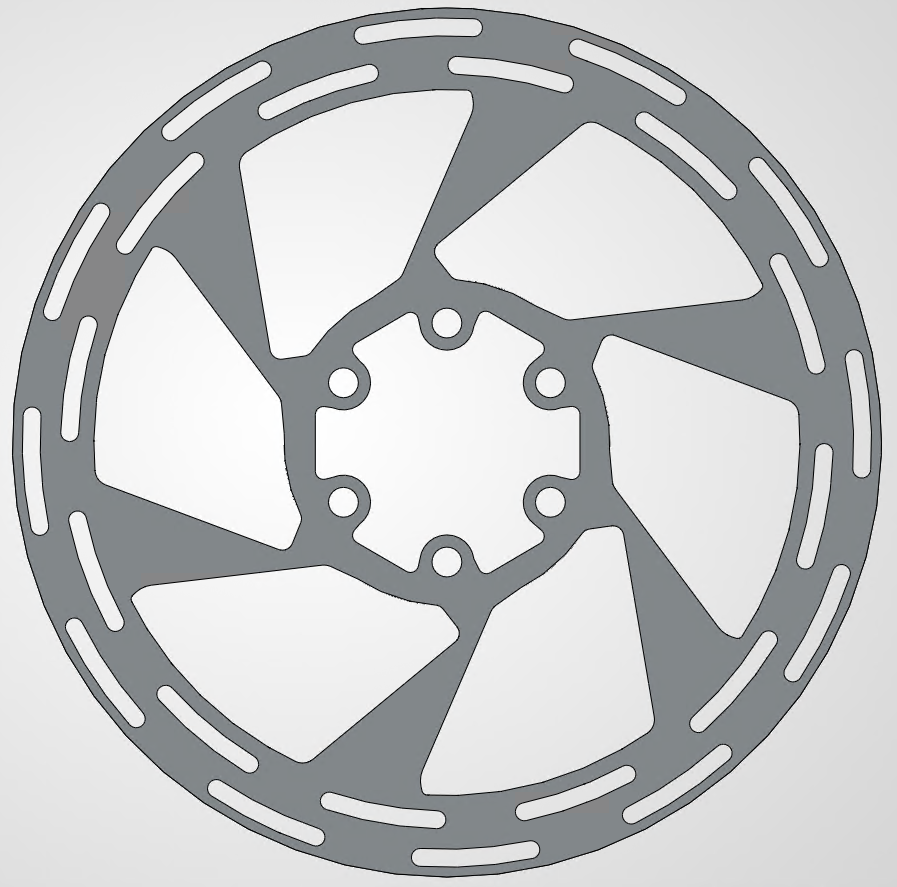
\includegraphics[width=\textwidth]{Figures/CADRotorFront.png}
        \caption{Front view.}
        \label{fig:baseline_front}
    \end{subfigure}
    \hfill
    \begin{subfigure}[c]{0.47\textwidth}
        \centering
        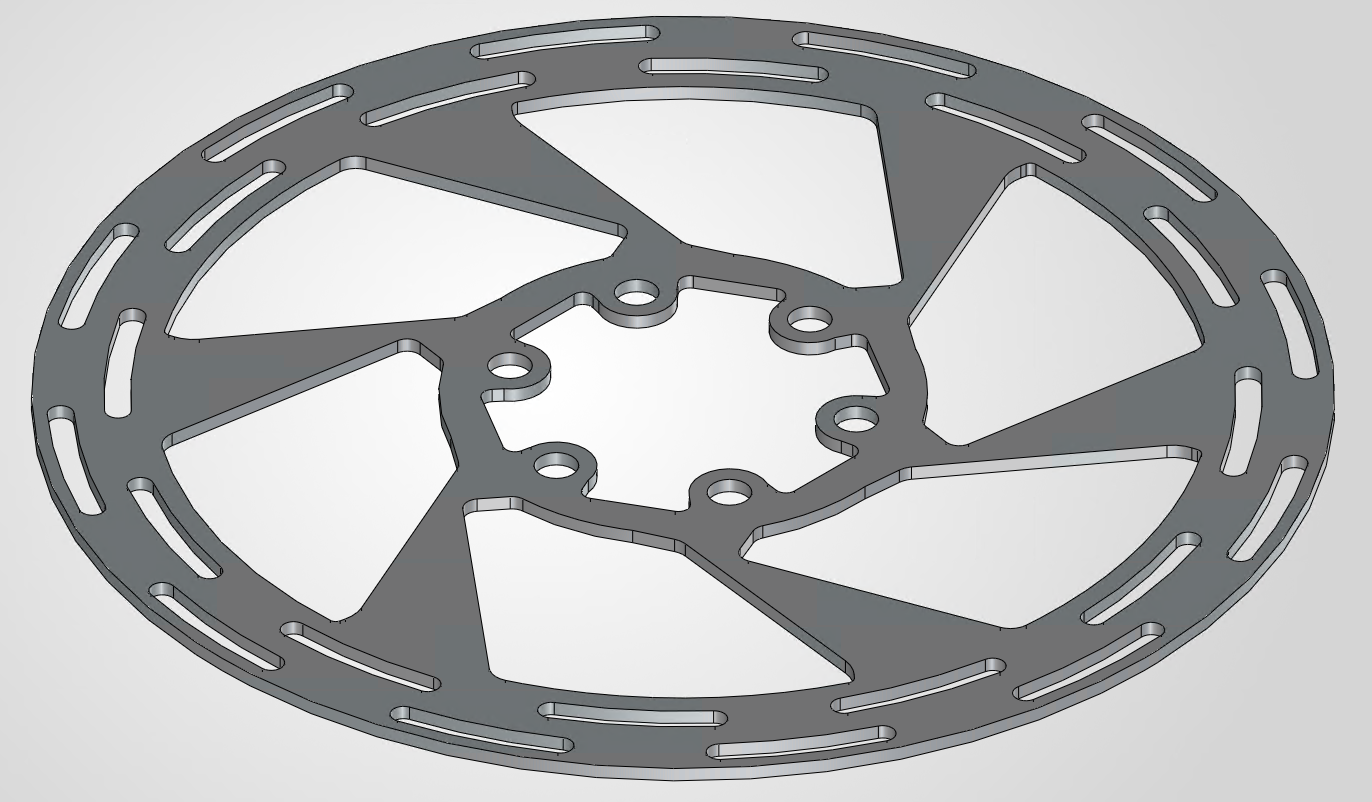
\includegraphics[width=\textwidth]{Figures/CADRotorIso.png}
        \caption{Isometric view.}
        \label{fig:baseline_iso}
    \end{subfigure}
    \caption{Simplified CAD model of the baseline 160~mm six-bolt disc-brake rotor.}
    \label{fig:baseline_cad}
\end{figure}

Using the assigned stainless-steel density, the final model produced a mass
of \SI{125.47}{g}, a volume of \SI{16085.78}{mm^3}, and a total surface area
of \SI{22798.84}{mm^2}. The calculated centre of mass was
$(0.00,-0.03,0.00)$~mm relative to the rotor centre, confirming that the
simplified geometry remained effectively rotationally balanced.

As a secondary validation of the geometric simplification, an independently
reported mass of approximately \SI{112}{g} is available for the commercial
160~mm six-bolt Paceline rotor \cite{MTBIKERPaceline}. The simplified model
is therefore approximately 12\% heavier than the reported commercial
component. This difference was considered acceptable given that the
non-published internal geometry was reconstructed from image data and the
model intentionally retains simplified structural webs for subsequent
comparative analysis.


\subsection{Material Model}

SRAM does not publicly specify the exact stainless-steel grade or heat
treatment used for the Paceline rotor. AISI~410 stainless steel
(EN~1.4006) was therefore adopted as a representative material for the
structural and thermal analyses. This grade has documented use in bicycle
disc-brake rotors \cite{WorldStainlessSports} and provides the combination of
strength, wear resistance and corrosion resistance expected for this
application.

The material properties adopted for the numerical model are summarised in
Table~\ref{tab:material_properties}. Density was retained at
\SI{7800}{kg.m^{-3}}, consistent with the SOLIDWORKS chrome-stainless-steel
material used to calculate the baseline CAD mass. The remaining mechanical
and thermal properties are based primarily on published AISI~410 data
\cite{Atlas410,NIST410}.

\begin{table}[H]
    \centering
    \caption{AISI 410 stainless-steel properties adopted for the numerical model.}
    \label{tab:material_properties}
    \begin{tabular}{l c c}
        \toprule
        Property & Symbol & Value \\
        \midrule
        Density
        & $\rho_m$
        & \SI{7800}{kg.m^{-3}} \\

        Young's modulus
        & $E$
        & \SI{200}{GPa} \\

        Poisson's ratio
        & $\nu$
        & 0.286 \\

        Coefficient of thermal expansion
        & $\alpha$
        & \SI{9.9e-6}{K^{-1}} \\

        Thermal conductivity
        & $k$
        & \SI{24.9}{W.m^{-1}.K^{-1}} \\

        Specific heat capacity
        & $c_p$
        & \SI{460}{J.kg^{-1}.K^{-1}} \\

        Conservative yield strength
        & $\sigma_y$
        & \SI{275}{MPa} \\
        \bottomrule
    \end{tabular}
\end{table}

Because the actual Paceline alloy condition is unknown, the minimum
annealed 0.2\% proof strength reported for AISI~410 is used as a conservative
yield criterion \cite{Atlas410}. The material properties are treated as
temperature-independent in the first-order numerical model. This
simplification is appropriate for the comparative design study, although the
temperature dependence of material properties should be considered in a
higher-fidelity rotor model.

\subsection{Thermal Model}

% Explain:
% - heat input
% - convection
% - initial temperature
% - simulation time
% - major assumptions

\todo{Document thermal boundary conditions.}


\subsection{Structural Model}

% Explain:
% - rotor constraint
% - braking torque
% - loading surface
% - outputs: von Mises stress and deformation

\todo{Document structural boundary conditions.}


\subsection{Mesh Verification}

% Keep this SIMPLE.
%
% Three meshes maximum:
% coarse / medium / fine
%
% Compare one useful quantity:
% peak temperature OR maximum stress.
%
% A short table + one sentence is enough.

\todo{Perform compact mesh sensitivity check.}


% ============================================================
\section{Design Development and Optimisation}
% ============================================================

\subsection{Design Variables}

% Keep the number of variables LOW.
%
% Possible variables:
% - cut-out geometry
% - cut-out size
% - web/spoke width
%
% Avoid trying to optimise everything.

\todo{Define the geometric parameters actually changed.}


\subsection{Candidate Designs}

% Aim for:
% Baseline
% Design A
% Design B
% Design C
%
% Show all four geometries in one figure if possible.

\todo{Create 2--3 realistic alternative rotor geometries.}


\subsection{Performance Comparison}

% This is probably the most important table in the report.

\begin{table}[H]
    \centering
    \caption{Comparison of baseline and candidate rotor designs.}
    \label{tab:design_comparison}
    \begin{tabular}{l c c c c}
        \toprule
        Design &
        Mass &
        $\Tmax$ &
        $\sigmavm,\max$ &
        Max. deformation \\
        \midrule

        Baseline & -- & -- & -- & -- \\
        Design A & -- & -- & -- & -- \\
        Design B & -- & -- & -- & -- \\
        Design C & -- & -- & -- & -- \\

        \bottomrule
    \end{tabular}
\end{table}


\subsection{Final Design Selection}

% Explain the trade-off.
%
% Do not simply state "Design C was best."
%
% Explain WHY:
% - X% lower mass
% - only Y% temperature increase
% - stress remains within limit
% etc.

\todo{Select final design using quantitative evidence.}


% ============================================================
\section{Results and Discussion}
% ============================================================

\subsection{Thermal Performance}

\todo{Discuss main thermal result.}


\subsection{Structural Performance}

\todo{Discuss main structural result.}


\subsection{Mass Reduction and Engineering Trade-Off}

\todo{Quantify improvement relative to baseline.}


\subsection{Model Limitations}

% Keep honest and specific.
%
% Examples:
% - simplified convection
% - assumed braking distribution
% - idealised contact between pad and rotor
% - constant material properties if applicable
% - no experimental validation

\todo{State the important limitations without undermining the entire project.}


% ============================================================
\section{Conclusions}
% ============================================================

% Aim for around 4--6 strong conclusions.
%
% Every conclusion should preferably contain a number.

\todo{
Summarise:
baseline result,
final geometry,
mass reduction,
thermal result,
structural result,
main engineering conclusion.
}


% ============================================================
% REFERENCES
% ============================================================

\bibliographystyle{unsrtnat}
\bibliography{references}


% ============================================================
% APPENDIX
% ============================================================

\appendix

\section{Additional Calculations}

% Put detailed derivations here if they interrupt the main report.


\section{Additional Simulation Results}

% Extra contour plots, mesh results etc.


\end{document}